\documentclass{article}
\usepackage{longtable}
\usepackage{makecell}
\usepackage{float}
\usepackage{graphicx}
\usepackage{bm}
\usepackage{placeins}
\usepackage{threeparttable} 
\usepackage{multirow}
\usepackage{aligned-overset}
\usepackage[slantfont,boldfont]{xeCJK}
\usepackage{fontspec}
\setCJKmainfont{SimSun}
\setmainfont{SimSun}
\setsansfont{SimSun}

\title{改装电表实验报告}
\author{2411545 邱凯锐}
\date{2025.3.10}

\begin{document}
\maketitle
\section{实验目的}
\hspace*{1em}1.掌握微电流表性能参数的测量方法。\\
\hspace*{1em}2.掌握直流指针式电流表和电压表的改装原理、校准曲线测量和刻度方法。\\
\hspace*{1em}3.掌握欧姆表的改装原理、调零方法和刻度方法。\\
\hspace*{1em}4.掌握仪表的校准测量方法,以及使用最大示值误差法确定仪表等级。

\section{实验原理}
\subsection{测量微电流表的性能参数:}
\hspace*{2em}微电流表的线圈有一定内阻,用$R_g$表示;微电流表允许通过的最大电流称为满度电流,用$I_g$表示;微电流表的准确度等级用$Q_g$表示。
微电流表的内阻$R_g$、满度电流$I_g$和准确度等级$Q_g$是表示其特性的三个重要参数。\\
\hspace*{2em}\textbf{1.测量微电流表内阻$R_g$和满度电流$I_g$常用方法有:}\\
\hspace*{2em}\textbf{替代法、中值法(半电流法)}\\
\hspace*{2em}替代法测量原理见Figure 1,中值法测量原理见Figure 2。图中$E$为直流电源电压,$R_2、R_w$为阻值可以调节的电阻箱。\\
\begin{figure}[ht]
    \centering
    \begin{minipage}{0.45\textwidth} % 调整宽度为总宽度的45%
        \centering
        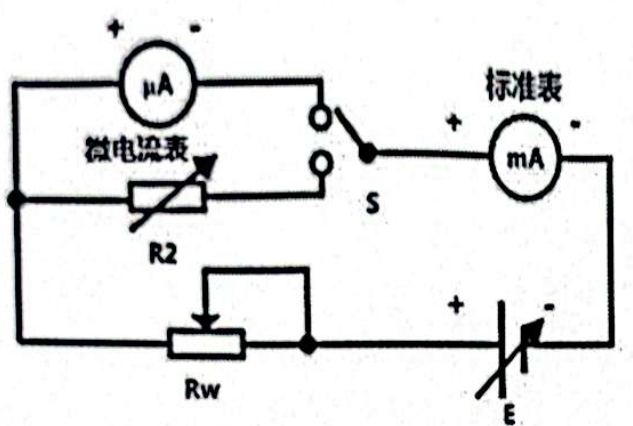
\includegraphics[width=3cm]{1.1.png} % 替换为你的图片路径
        \caption{替代法原理图}
    \end{minipage}\hfill
    \begin{minipage}{0.45\textwidth}
        \centering
        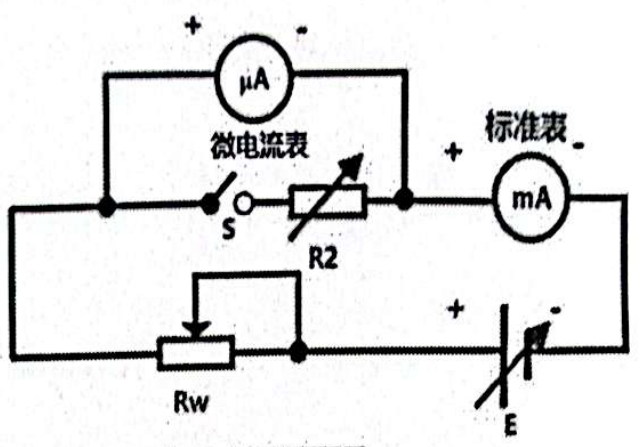
\includegraphics[width=3cm]{1.2.png} % 替换为你的图片路径
        \caption{中值法原理图}
    \end{minipage}
\end{figure}
\\
\hspace*{2em}\textbf{2.仪表准确度等级:}\\
\hspace*{2em} 仪表的准确度等级有0.1、0.2、0.5、1.0、1.5、2.5、5.0七个等级。用最大示值误差的绝对值除以仪表量程的百分比,即为仪表的准确度等级。
$$
Q \% =\frac{\Delta X_m}{X_m}\times 100 \%
$$
\hspace*{2em} 仪表的准确度等级可以由其校准曲线获得。

\subsection{将微电流表改装成大量程电流表:}
\hspace*{2em}Figure 3为改装电流表的原理图。这种由微电流表和并联电路$R_2$组成的整体(图中虚线框住的部分)就是改装后的电流表。如需将量程扩大为原来的$n$倍,则不难得出:
$$
R_2=R_g/(n-1)
$$
\begin{figure}[ht]
    \centering
    \begin{minipage}{0.45\textwidth} % 调整宽度为总宽度的45%
        \centering
        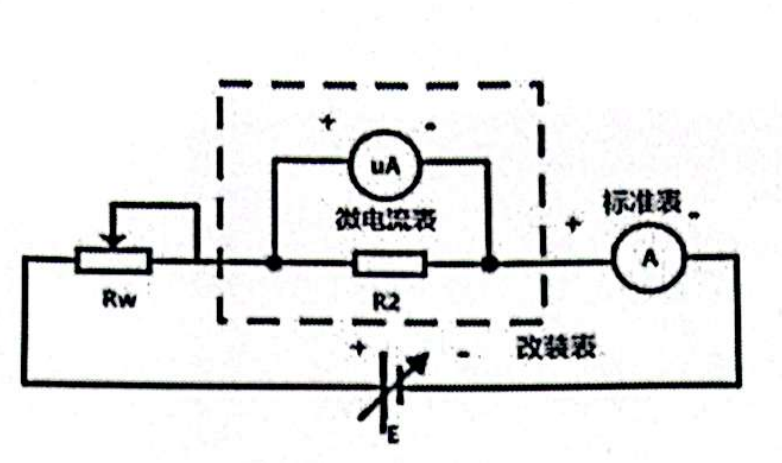
\includegraphics[width=3cm]{1.3.png} % 替换为你的图片路径
        \caption{改装电流表实验线路图}
    \end{minipage}\hfill
    \begin{minipage}{0.45\textwidth}
        \centering
        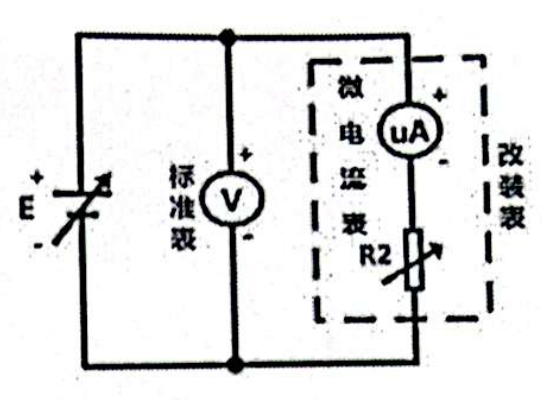
\includegraphics[width=3cm]{1.4.png} % 替换为你的图片路径
        \caption{改装电压表实验线路图}
    \end{minipage}
\end{figure}
\subsection{将微电流表改装成电压表:}
\hspace*{2em}Figure 4为改装电压表原理图。这种由微电流表和串联电阻$R_2$组成的整体就是改装电压表。选取不同大小的$R_2$,就可以得到不同量程的电压表。如果改装电压表的量程为$U$,通过微电流表的最大电流为$I_g$,改装电压表的内阻为$U/I_g$,因此需要串联的分压电阻$R_2$的阻值为:
$$
R_2=\frac{U}{I_g}-R_g
$$ 

\subsection{将微电流表改装成欧姆表:}
\hspace*{2em}用来测量电阻大小的电表称为欧姆表。根据调零方式的不同,可分为串联分压式和并联分流式两种。其原理电路如Figure 5所示。
\begin{figure}[h]
    \centering
    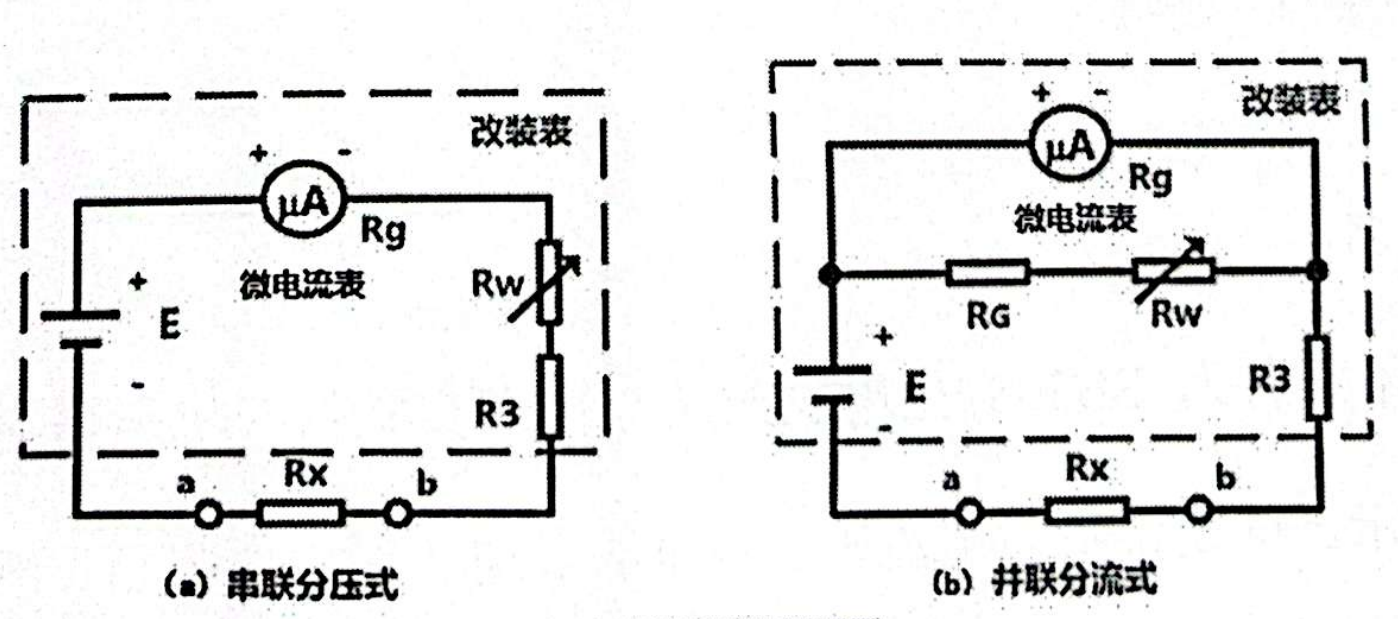
\includegraphics[width=8cm]{1.5.png}
    \caption{欧姆表改装原理图}
\end{figure}
\hspace*{2em}Figure 5中$E$为电源电压,$R_3$为限流电阻,$R_W$为调“零”电阻,$R_X$为待测电阻,$R_g$为微电流表内阻。在Figure 5(a)中,当a、b端接入被测电阻$R_X$后,电路中的电流为:
$$
I=\frac{E}{R_g+R_W+R_3+R_X}
$$
\hspace*{2em}当电源端电压$E$保持不变时,被测电阻和电流值有一一对应的关系。$R_X$越大,电流$I$越小。短路a、b两端,即$R_X=0$时:
$$
I=\frac{E}{R_g+R_W+R_3}=I_g
$$
当 $R_X=R_g+R_W+R_3$时:
$$
I=\frac{E}{R_g+R_W+R_X+R_3}=\frac{1}{2}I_g
$$
这是指针在微电流表的中间位置,对应的阻值为中值电阻,显然$R_{中}=R_g+R_w+R_3$。\\
\hspace*{2em}当$R_X=\infty $时,$I=0$,即指针在微电流表的机械零位。\\
\hspace*{2em}综上所诉,欧姆表的标度尺为反向刻度,且刻度是不均匀的。

\section{实验设备}
\hspace*{2em}实验用设备为 FB308 型电表改装和校准实验仪(杭州经科仪器有限公司),如Figure 6所示。
\begin{figure}[h]
    \centering
    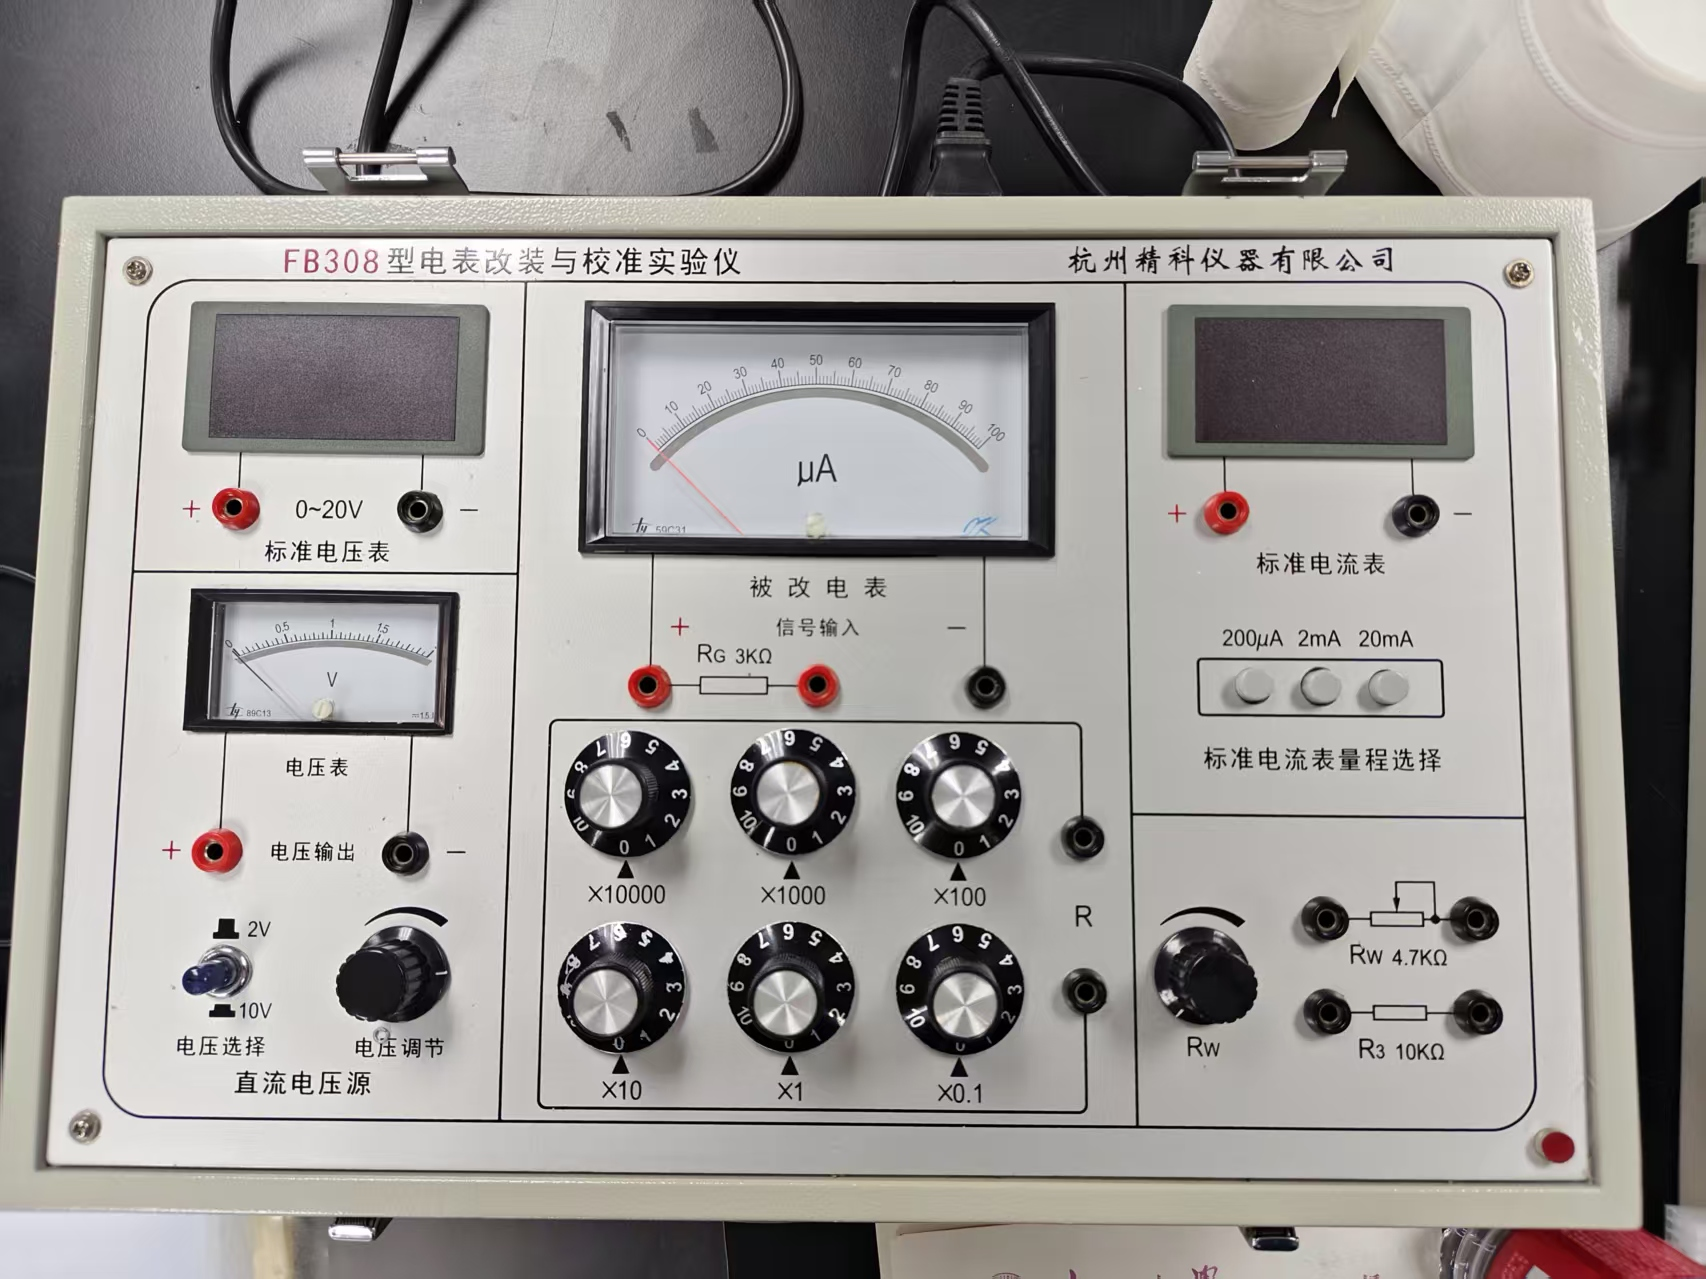
\includegraphics[width=7cm]{2.1.jpg}
    \caption{仪器设备版面图}
\end{figure}
\\
\hspace*{2em}1.直流电压源:电压源有$0 \sim 2\,\mathrm{V}$、$0 \sim 10\, \mathrm{V}$两档,输出电压可连续调节。\\
\hspace*{2em}2.微电流表:量程约$100\, \mu\mathrm{A}$,内阻约$1.6k\Omega$,准确度等级为1.5级。\\
\hspace*{2em}3.标准电压表:量程$20 \mathrm{V}$,四位半数字式电压表,准确度等级为0.1级。\\
\hspace*{2em}4.标准电流表:三个量程:$200 \, \mathrm{\mu A},2 \, \mathrm{mA},20\, \mathrm{mA}$,准确度等级为0.1级。\\
\hspace*{2em}5.电阻箱 R:$0\sim 11111 \Omega$,分辨率 $0.1\Omega$ \\
\hspace*{2em}6.外电源:AC 220V$\pm 10\%,50\,\mathrm{Hz}$。

\section{实验内容}
\subsection{测量微电流表相关参数}
\hspace*{2em}\textbf{1.测量微电流表满度电流$I_g$}\\
\hspace*{2em}(1)按照电路图,依次串联电源、滑动变阻器$R_W$、微安表和标准表。
\hspace*{2em}(2)将电源电压调至$0.5\: \mathbf{V}$。调节滑动变阻器$R_W$,使微安表满偏(指针指最大量程),读取标准表读数,即为微安表满度电流$I_g$。\\
\hspace*{2em}\textbf{2.用替代法测量微电流表内阻$R_{g1}$}\\
\hspace*{2em}(1)按照电路图连接电路,将电源电压调至$0.5\: \mathbf{V}$。开关断开 $R_2$,接入微电流表,调节滑动变阻器$R_W$使微电流表满偏,记录标准表读数。\\
\hspace*{2em}(2)保持$R_W$不变,开关断开微电流表,连接电阻箱$R_2$,调节$R_2$阻值,使标准表读数与步骤(1)中相等。此时$R_2$阻值等于微电流表的内阻$R_{gII}$。\\
\hspace*{2em}\textbf{3.用中值法测量微电流表内阻$R_{g2}$}\\
\hspace*{2em}(1)按照电路图连接电路,将电源电压调至$0.5\: \mathbf{V}$。开关断开$R_2$,调节滑动变阻器$R_W$使得微电流表满度,记录此时标准表的读数。\\
\hspace*{2em}(2)开关闭合,将电阻箱$R_2$接入电路,通过调节滑动变阻器$R_W$和电阻箱$R_2$的阻值,同时满足标准表读数和步骤(1)中相等、微电流表指针指中值。此时电阻箱$R_2$的阻值大小等于微电流表的内阻$R_{g2}$。计算$R_{g2}$相对于$R_{g1}$的误差。

\subsection{改装成 $1\: \mathbf{mA}$ 量程的改装电流表}
\hspace*{2em}\textbf{1.根据电路参数计算出分流电阻阻值。}\\
\hspace*{2em}\textbf{2.用标准电流表改装电流表并且记下标准电流表相应的读数。}\\
\hspace*{2em}(1)按照电路图连接电路,调节电源电压至$0.5\: \mathbf{V}$。将电阻箱阻值设置为分流电阻阻值。\\
\hspace*{2em}(2)调节滑动变阻器$R_W$,使改装电流表的指针分别指$0.2\, \mathbf{mA}、0.4\,\mathbf{mA}、0.6\,\mathbf{mA}、\\0.8\,\mathbf{mA}、1.0\,\mathbf{mA}$。读取并记录相应的标准电流表读数。\\
\hspace*{2em}\textbf{3.根据数据,绘制改装电表的校准曲线,确定改装电流表的准确度等级。}

\subsection{改装成$1.5\, \mathbf{V}$量程的改装电压表}
\hspace*{2em}\textbf{1.根据电路参数计算扩程电阻阻值。}\\
\hspace*{2em}\textbf{2.用标准电流表改装电压表并且记下标准电压表相应的读数。}\\
\hspace*{2em}(1)按照电路图连接电路,调节电源电压至$1.5\: \mathbf{V}$。将电阻箱阻值设置为扩程电阻阻值。\\
\hspace*{2em}(2)调节电源电压,使改装电压表的示数分别指$0.3\, \mathbf{V}、0.6\,\mathbf{V}、0.9\,\mathbf{V}、1.2\,\mathbf{V}、\\1.5\,\mathbf{V}$。读取并记录相应的标准电压表读数。\\
\hspace*{2em}\textbf{3.根据数据,绘制改装电表的校准曲线,确定改装电压表的准确度等级。}

\subsection{改装欧姆表并标定表面刻度:}
\hspace*{2em}\textbf{1.按照串联分压式电路图连接电路,调节电源电压至1.5V}。\\
\hspace*{2em}\textbf{2.将欧姆表进行调零。}\\
\hspace*{2em}(1)对于欧姆表来说,最大刻度对应电路的断路,也就是待测电阻无穷大,这时微安表上没有电流流过;零刻度对应待测的短路,电阻无穷小,这时需要调节控制使微安表满度,即为调零。\\
\hspace*{2em}(2)操作上,将待测电阻$R_x$短路,调节滑动变阻器$R_w$,使微安表满度,此时电路中电流等于欧姆表电流,电路中电阻等于欧姆表的内阻。\\
\hspace*{2em}\textbf{3.测量改装成的欧姆表的中值电阻$R_中$。}\\
\hspace*{2em}将$R_x$接入电路,调节$R_x$阻值,当$R_x$的阻值等于欧姆表内阻时,电路中的电流等于被该表满度电流的一半,此时$R_x$的阻值称为中值电阻。\\
\hspace*{2em}\textbf{4.绘制出改装成欧姆表的标度盘。}\\
\hspace*{2em}分别将中值电阻、中值电阻的1/2、1/3、1/4、1/5、2、3、4、5倍接入电路,读取电流表指针偏离中间刻度的格数(估读一位),以此为基础,绘制表盘刻度。\\
\hspace*{2em}\textbf{5.确定改装成的欧姆表的电源电压使用范围。}\\
\hspace*{2em}欧姆表电源电压的使用范围,就是欧姆表的可调零范围。操作中,将$R_x$短路,分别将$R_w$的阻值调至最小和最大值,对应可以使被改表满偏的电源电压范围,即为电源电压的可用范围。

\section{实验数据}
\subsection{微电流表相关参数}
\begin{longtable}{cccc}
    %\centering
    \caption[Short Caption]{$微电流表相关参数$}
    \renewcommand{\arraystretch}{1.2}
    \label{table:longtable_example} \\
    % 下面是表头
    \hline  满度电流$I_g(\mathbf{\mu A})$ & 替代法$R_{g1}(\Omega)$ & 中值法$R_{g2}(\Omega$) & $|R_{g1}-R_{g2}|$ \\ \hline 
    \endfirsthead
    % 下面数字3的意思是表格的列数
    \multicolumn{4}{c}%
    {{\bfseries \tablename\ \thetable{} -- continued from previous page}} \\
    \hline  满度电流$I_g/\mathbf{\mu A}$ & 替代法$R_{g1}/\Omega$ & 中值法$R_{g2}/\Omega$ & $|R_{g1}-R_{g2}|$ \\ \hline 
    % 注意这里把表头复制了一遍,因为在新的页面也会展示一下表头,不然表格不方便阅读
    \endhead
    \hline \multicolumn{4}{r}{{Continued on next page}} \\ \hline
    \endfoot
    \hline \hline
    \endlastfoot
    99.87    & 1955.0    & 1958.4    & 3.4 \\ \hline
    \end{longtable}

\subsection{改装成$1\, \mathbf{mA}$电流表}
\begin{table*}[h]
    \centering
    \renewcommand{\arraystretch}{1.2}
    \caption{改装电流表校准数据}
    \vspace{8pt}
    \label{table1}
    \begin{tabular}{cc|c|cc}
        % \caption[Short Caption]{$微电流表相关参数$}
        \hline
        \multirow{2}{*}{改装表读数\(I\)(mA)} & \multicolumn{3}{c}{标准表读数\(I_s\)(mA)} & \multirow{2}{*}{误差\(\Delta I\)(mA) }\\
        \cline{2-4} 
         & 递减时 & 递增时 & 平均值 &  \\
         \hline
         0.2   & 0.2004 & 0.2032 & 0.2018 & 0.0018 \\ \hline
         0.4   & 0.3996 & 0.3994 & 0.3995 & 0.0005  \\ \hline
         0.6   & 0.5989 & 0.5989 & 0.5989 & 0.0011  \\ \hline
         0.8   & 0.7989 & 0.8025 & 0.8007 & 0.0007  \\ \hline
         1.0   & 1.0070 & 0.9996 & 1.0033 & 0.0033 \\ \hline  
        \hline
        \end{tabular}    
\end{table*}
计算可得,$Q=0.33$,从而确定准确度等级为0.5,校准曲线如Figure 7所示。
\begin{figure}[H]
    \centering
    \begin{minipage}{0.45\textwidth} % 调整宽度为总宽度的45%
        \centering
        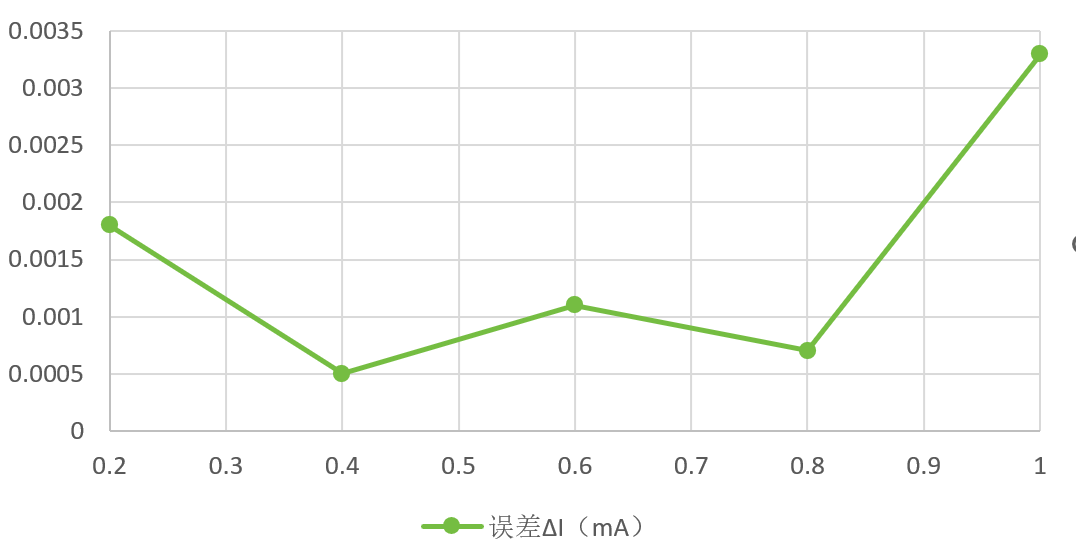
\includegraphics[width=6cm]{3.1.png} % 替换为你的图片路径
        \caption{改装电流表校准曲线}
    \end{minipage}\hfill
    \begin{minipage}{0.45\textwidth}
        \centering
        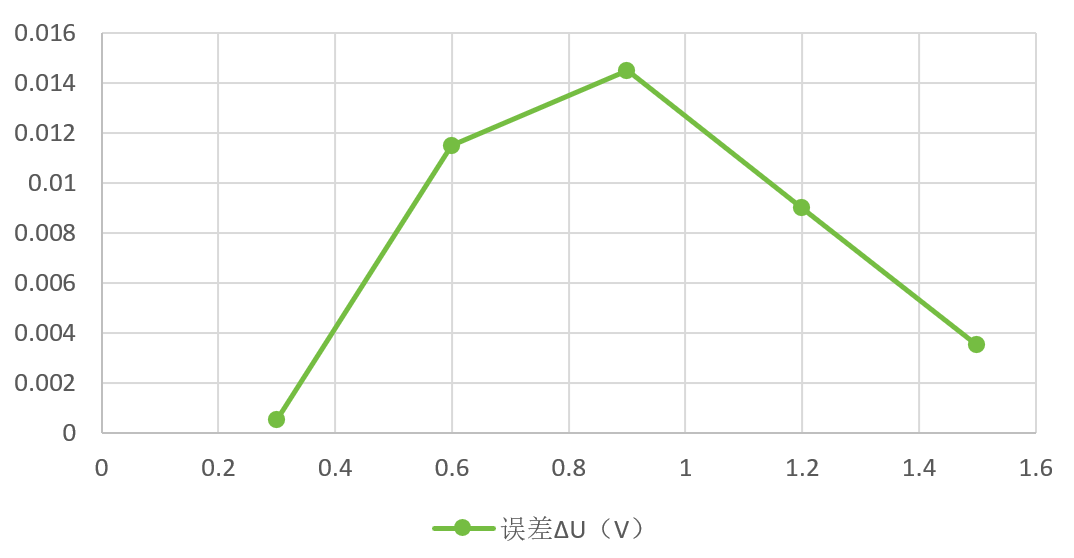
\includegraphics[width=6cm]{3.2.png} % 替换为你的图片路径
        \caption{改装电压表校准曲线}
    \end{minipage}
\end{figure}
\subsection{改装成$1.5\,\mathbf{V}$量程的改装电压表}
\begin{table*}[h]
    \centering
    \caption{改装电压表校准数据}
    \renewcommand{\arraystretch}{1.2}
    \vspace{8pt}
    \label{table1}
    \begin{tabular}{ccccc}
        % \caption[Short Caption]{$微电流表相关参数$}
        \hline
        \multirow{2}{*}{改装表读数\(U\)(V)} & \multicolumn{3}{c}{标准表读数\(U_s\)(V)} & \multirow{2}{*}{误差\(\Delta U\)(V) }\\
        \cline{2-4} 
         & 递减时 & 递增时 & 平均值 &  \\
         \hline
         0.3   & 0.298 & 0.301 & 0.2995 & 0.0005 \\ \hline
         0.6   & 0.587 & 0.590 & 0.5885 & 0.0115  \\ \hline
         0.9   & 0.882 & 0.889 & 0.8855 & 0.0145  \\ \hline
         0.12  & 1.191 & 1.191 & 1.191  & 0.0090  \\ \hline
         0.15  & 1.496 & 1.497 & 1.4965 & 0.0035 \\ \hline \hline
        \end{tabular}    
\end{table*}
计算可得:$Q=0.97$,从而确定的准确度等级为1.0,校准曲线如Figure 8所示。

\subsection{改装欧姆表并标定表面刻度}

\begin{table*}[h]
    \centering
    \renewcommand{\arraystretch}{1.2}
    \begin{tabular}{ccc} 
        \hline
        \multirow{2}{*}{中值电阻$R_中(\Omega)$} & \multicolumn{2}{c|}{电源电压可用范围 $E(\mathbf{V})$}\\
        \cline{2-3} 
         & $E_{\min}$ & $E_{\max}$  \\
        \hline
        15550.5 & 1.180 & 1.695\\ \hline
        \hline
        \end{tabular}    
\end{table*}

\begin{table*}[h]
    \centering
    \renewcommand{\arraystretch}{1.5}
    \caption{欧姆表改装数据}
    \label{table1}
    \vspace{8pt}
    \begin{threeparttable}
    \begin{tabular}{cccccccccc} 
        \hline
        $R_{X_i}(\Omega)$ & $\frac{1}{5}R_中$ & $\frac{1}{4}R_中$ & $\frac{1}{3}R_中$ & $\frac{1}{2}R_中$ & $R_中$ & $2R_中$ & $3R_中$ & $4R_中$ & $5R_中$  \\ 
        \hline
        偏转格数(div) & +33.1 & +29.9 & +25.1 &+16.8 & 0 &-17&-25.2&-30.5&-34\\ \hline
        \hline
        \end{tabular}    
    \begin{tablenotes}
        \footnotesize               %这行要添加
        \item[1]  +表示指针向右偏转,-表示向左         %这行要添加
    \end{tablenotes}
    \end{threeparttable}
\end{table*}

\begin{figure}[h]
    \centering
    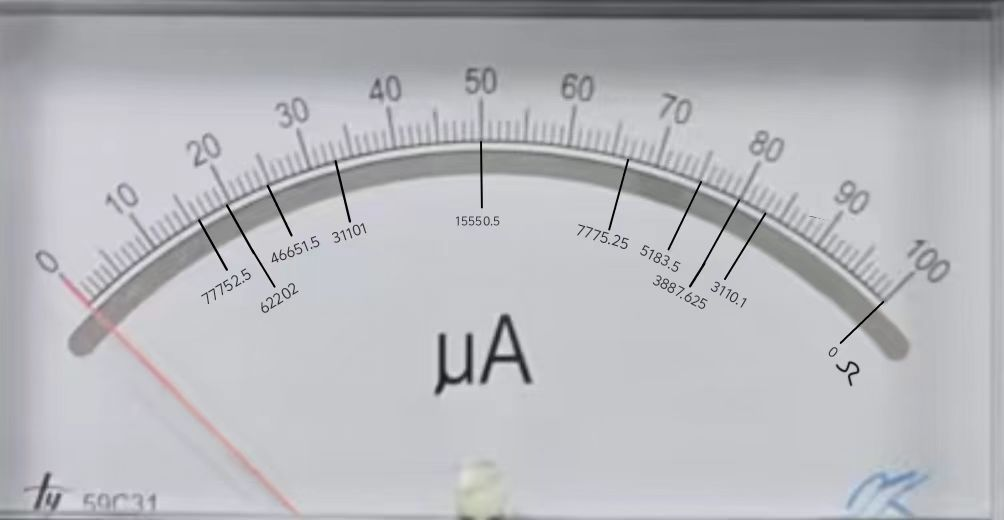
\includegraphics[width=9cm]{3.3.jpg}
    \caption{改装欧姆表标度盘}
\end{figure}

\section{思考题}
(1)\textbf{用替代法和中值法测量微电流表内阻,哪种方法更为准确?为什么?如何修正相对不准确方法得到的结果?}\\
\hspace*{2em}替代法更为准确。因为替代法在调节接入电阻箱$R_2$阻值的过程中,操作简单,其他电路参数相对稳定,
同时测量进度主要受限于电阻箱和标准电流表的精度,而中值法需要同时调节滑动变阻器$R_W$和电阻箱$R_2$,操作更为复杂,电路改变的程度更大,测量精度还额外受限于表头的精度和人为读数判断。
\hspace*{2em}修正方法为多次测量求平均值,同时适当改变电源电压,得到不同外电路环境下的数据,从而减小误差。\\
(2)\textbf{测量校准曲线过程中为何要在改装表示数递增与递减方向上各测一遍?}
\hspace*{2em}微安表的机械结构可能额外受到电磁力矩和摩擦力矩的影响,指针在不同变化方向上的示数存在差异,所以需要同时测量递增和递减方向上的数据,求平均值,从而减小误差。\\
(3)\textbf{为什么需要测量改装欧姆表的电源电压适用范围?测量原理是什么?}\\
\hspace*{2em}只有在电源电压在使用范围内的时候,才可以通过调节滑动变阻器使得微安表满偏,即欧姆表调零。原理为$Ig=\frac{E}{R_g+R_3+R_w}$,分别测量$R_w$为最小值0和最大值$R_{w_{\max}}$下,使得式子成立的电源电压$E_{\min}$和$E_{\max}$。$E_{\min}\sim E_{\max}$即为电源电压适用范围。
\section{总结}
\hspace*{2em}通过本次实验,我们对微安表的结构原理、性能参数和改装方法有了更深入的理解,并且较为成功的测定了相关的实验数据。\\
\hspace*{2em}同时我们掌握了替代法和中值法以测量微安表内阻,以及通过测量递增和递减两个方向上的数据,来减小微安表机械结构导致的误差的方法,对日后相关实验有一定的帮助。
\end{document}